% !TeX spellcheck = de_AT_frami
\section{Numerische Differentiation}
	\begin{enumerate}
		\item \textbf{Wie wird mit Hilfe der Vorwärtsdifferenz eine differenzierbare Funktion \(\mathbf{f}\) an der Stelle \(\mathbf{x}\) differenziert? Wie groß ist \(\mathbf{\text{h}_{\text{opt}}}\)?}
			\begin{align*}
				f(x)=\frac{f(x+h)-f(x)}{h}-\frac{h}{2}f''(\xi), \quad \text{h}_{\text{opt}}=\sqrt{\texttt{eps}}
			\end{align*}
		\item \textbf{Wie wird mit Hilfe der zentralen Differenz eine differenzierbare Funktion \(\mathbf{f}\) an der Stelle \(\mathbf{x}\) differenziert? Wie groß ist \(\mathbf{\text{h}_{\text{opt}}}\)}
			\begin{align*}
				f(x)=\frac{f(x+h)-f(x-x)}{2h}-\frac{h^2}{6}f'''(\xi), \quad \text{h}_{\text{opt}}=\sqrt[3]{\texttt{eps}}
			\end{align*}
		\item \textbf{Wie verhalten sich Verfahrensfehler und Rundungsfehler in Abhängigkeit von der Schrittweite \(\mathbf{h}\)? Machen Sie eine Skizze.}
			\begin{figure}[!htbp]
				\centering				
				\begin{minipage}{.4\textwidth}
					\centering
					\begin{align*}
						|V(h)|&\leq C_\text{V} h \\
						|R(h)|&\leq C_\text{R} \frac{\texttt{eps}}{h} \\
						|\text{err}(h)|&\leq C_\text{V} h + C_\text{R} \frac{\texttt{eps}}{h}
					\end{align*}
				\end{minipage} %				
				\begin{minipage}{.5\textwidth}
					\centering
					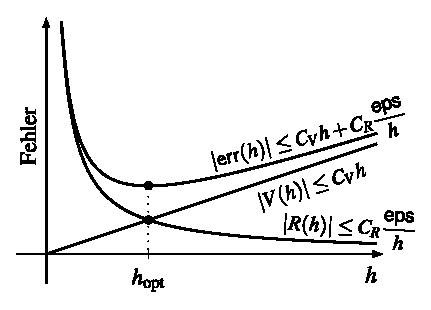
\includegraphics[width=0.8\linewidth]{Kap2_1}
				\end{minipage}
			\end{figure}			
		\item \textbf{Wie lässt sich mit Hilfe eines logarithmischen Plots das Verhalten von Verfahrensfehler und Rundungsfehler ablesen? Wie kann man die optimale Schrittweite \(\mathbf{h_{opt}}\) ablesen?}
			\begin{align*}
				\log |\text{err}|=\log \left( C_\text{V} h + C_\text{R} \frac{\texttt{eps}}{h}\right) \approx 
					\begin{cases}
						\log\left(C_\text{R}\texttt{eps}h^{-q}\right) =-q\log h + \log C_\text{R}+\log\texttt{eps}  , & \text{links von }  \text{h}_\text{opt},\\
						\log\left(C_\text{V}\texttt{eps}h^p\right) =p\log h + \log C_\text{V} , & \text{rechts von }  \text{h}_\text{opt}.		\\	
					\end{cases}
			\end{align*}
			Somit erhält man zwei Geraden der Form \(y=kx+d\), wobei \(k=-\text{q}\) und \(k=\text{p}\) aus dem Plot abgelesen werden können.\\
			Die optimale Schrittweite kann man im Schnittpunkt der beiden Geraden erkennen. 
		\item \textbf{Wieso gilt bei der zentralen Differenz für den Verfahrensfehler \(\mathbf{V(h)=\mathcal{O}(h^2)}\) statt \(\mathbf{\mathcal{O}(h)}\)?}\\
			Für die zentrale Differenz werden die Taylorpolynome für \(f(x+h)\) und \(f(x-h)\) gemittelt. Dabei heben sich die Terme zweiter Ordnung, \(\frac{h^2}{2}f''(x)\), auf.
		\item \textbf{Wie wird die zweite Ableitung einer zweimal differenzierbaren Funktion an der Stelle \(\mathbf{x}\) berechnet? Wie groß ist \(\mathbf{h_{opt}}\)?}
			\begin{align*}
				f''(x)=\frac{f(x+h-2f(x)+f(x-h)}{h^2}-\frac{h^2}{12}f^{(4)}(\xi), \quad \text{h}_\text{opt}=\sqrt[\left( \text{q}+\text{p}\right) ]{\texttt{eps}}=\sqrt[4]{\texttt{eps}}
			\end{align*}
		\item \textbf{Wie lässt sich die optimale Schrittweite \(\mathbf{h_{opt}}\) aus dem Verfahrensfehler \(\mathbf{V(h)}\) und dem Rundungsfehler \(\mathbf{R(h)}\) bestimmen?}
			\begin{align*}
				|\text{err}(h)|&\leq C_\text{V} h + C_\text{R} \frac{\texttt{eps}}{h}
			\end{align*}
			Der Fehler soll minimal sein und somit \(C_\text{V} h + C_\text{R} \frac{\texttt{eps}}{h}=\text{min}.\) Dies führt zu \(C_\text{V} h^2 + C_\text{R}\texttt{eps}=0\) und somit
			\begin{align*}
				\text{h}_\text{opt}=\sqrt{\texttt{eps}\frac{C_\text{V}}{C_\text{R}}}.
			\end{align*}			 
			Bei \(f(x)\approx f'(x) \approx f''(x)\) gilt \(C_\text{V} \approx C_\text{R}\) und somit
			\begin{align*}
				\text{h}_\text{opt}&=\sqrt{\text{eps}}
			\end{align*}
		\item \textbf{Wie berechnet man die Jacobimatrix einer vektorwertigen Funktion \(\mathbf{f:}{\rm I\!R}\mathbf{^n} \rightarrow {\rm I\!R}\mathbf{^m}\) durch numerisches Differenzieren?}\\
			Jacobimatrix: \(\mathbf{J(x)}=\mathbf{f'(x)})=\begin{bmatrix}
				\pd{f_1}{x_1} & \cdots & \pd{f_1}{x_n} \\
				\vdots &  & \vdots \\
				\pd{f_{m}}{x_1} & \cdots & \pd{f_m}{x_n}
			\end{bmatrix}\) \\\\
			Approximation der i-ten Spalte
			\begin{align*}
				\pd{\mathbf{f}}{x_i}(\mathbf{x})=
					\begin{bmatrix}
						\pd{f_1}{x_i}(\mathbf{x}) \\
						\vdots \\
						\pd{f_m}{x_i}(\mathbf{x})
					\end{bmatrix}
					\approx \frac{\mathbf{f}(x_1,\dots,x_{i-1},x_i+h,x_{i+1},\dots,x_n)-\mathbf{f(x)}}{h}
			\end{align*}
		\item \textbf{Wie berechnet man den Gradient einer skalaren Funktion \(\mathbf{f:}{\rm I\!R}\mathbf{^n} \rightarrow {\rm I\!R}\mathbf{^m}\) durch numerisches Differenzieren?}\\
	\end{enumerate}